\documentclass[main.tex]{subfiles} 

\begin{document}
\section*{Analyse}
\label{sec:2}
Hvordan ble undervisningen lagt opp for å danne begrepsforståelse i naturfagstimene?

%IRE/F metoden <legg til forklaring> brukes, der elevene som rekker opp hånda blir spurt. Det viser seg at det 
%er noen få elever, som viser trygghet og kontroll når de responderer til lærer initiert dialog. 

% En av de viktigste egenskapene en lærer kan utvise er evnen til å tilpasse seg overfor 
% klassen, en gruppe eller på individnivå.<må begrunnes fra litteratur> 
% Ved å være bevisst på at alle elevene skal ha kjennskap til 
% begrepene som blir tatt opp og repetert, er det da nødvendig å få bekreftet at elevene innehar en 
% overordnet forståelse. Det kan derfor være nødvendig å utpeke noen elever som ikke viser aktiv 
% deltagelse i timen og frembringe deres respons. Dette er problematisk hvis det viser seg at 
% de ikke har forutsetninger for å kunne respondere. Da settes de i en vanskelig situasjon læreren 
% må lede de ut av, for eksempel ved hjelp av ledende spørsmål. Hvis det derimot 
% er forventet at det er en del av forutsetningene at elevene skal kunne respondere på lærer 
% initiativ, kan utspørringen av elevene vise hull i deres kunnskap. I 2. time blir en 
% annen form for lærerinitiativ brukt til å frembringe respons. 

% En viktig del av den sosiale utprøvingen av ideer og begreper innebærer å sammenlikne egne forestillinger
% med andres forestillinger i tillegg til naturvitenskapens forklaringer 
\citeA{odeg10}\citeA{dals94}

% Mortimer og Scott (2003) beskriver for eksempel læring som både individuell meningsskaping
% hvor man rekonstruerer gamle og nye ideer, og dialogisk meningsskaping hvor ideer gis et språk
% i en sosial sammenheng. Her skapes mening ved at man får forståelse av faglig kunnskap; i første
% rekke begrepsforståelse. 
\citeA{odeg10}

\begin{figure}[h!]
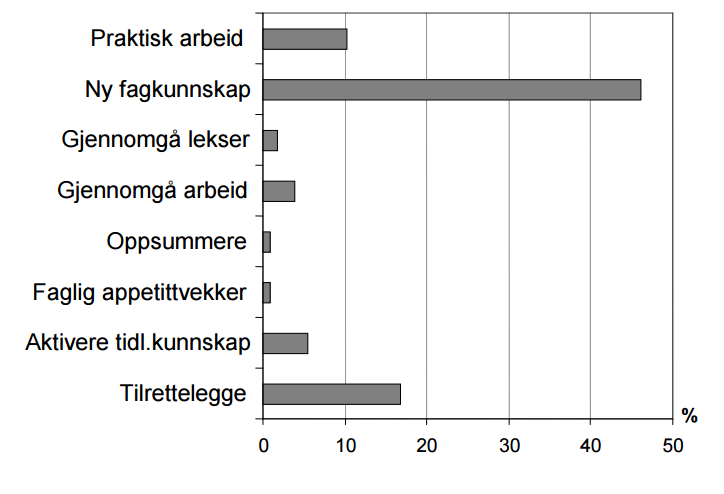
\includegraphics[scale = 0.6]{../figures/undervisnings_aktivitet.png}
\caption{Oversikt over lærernes undervisningstilbud til elevene i prosent av kodet tid. Kilde: \protect\citeA{odeg10}.}
\label{fig:odeg10}
\end{figure}

% gode fagsentrerte samtaler mellom elever hvor elever brukte egne erfaringer
% og språket for å oppnå faglig forståelse, eller faglige samtaler med lærer som hjelper til å skape
% bro mellom praksis og teori 
\citeA{odeg10}


%  ”inquiry-based science teaching” 
\citeA{knai11}

%Siden resterende del av timen skal brukes til repetisjon, er det ikke nødvendig å 
%prøve å finne svakheter i elevenes respons gjennom helklassesamtalen. For å finne slike svakheter 
%ble gruppesamtalene en bedre plattform. I den forbindelse ble tokolonnenotatet tatt i bruk (se 
%vedlegg : \ref{sec:tokolonnenotat}).

% Timen 2. starter på tilsvarende vis som den første timen. Derimot i denne timen er oppsettet 
% forskjellig. Hensikten med timen er å repetere leksene elevene har fått til timen, om celletyper og
% utvikling av celler fra enkeltceller til flercelledeorganismer. Etter å konsultert med veilederen
% var jeg nå klar over at alle elevene hadde forutsetning til å kunne respondere til våre spørsmål, 
% så lenge de var relatert til leksene. Etter den første timen var jeg nå bevisst på at elevenes 
% respons var avhengig av deres trygghet med et gitt tema. 

% Til den siste timen hadde vi innsamlet prøver fra en utflukt og lagret de i laboratoriet. 
% Gjennom tilstrekkelige forhold hadde vi klart å vokse fram encellede organismer, deriblant tøffeldyr 
% (en organisme som er oppkalt etter sko fordi dens utseende ligner på tøfler).

Et premiss for dybdelæring er at elevene får anvendt kunnskapen, og dermed opplever de større grad av faglig utvikling, \citeA{beer14}.


\end{document}
